\documentclass[twoside,11pt]{article}
\usepackage{blindtext}
\usepackage{algorithm}
\usepackage{algpseudocode}
\usepackage{amssymb}
\usepackage{caption}
\usepackage{svg}
\usepackage[preprint]{styles/jmlr2e}

\newcommand{\algorithmautorefname}{Algorithm}

\begin{document}

\title{Investigating and Combining Approaches for Data-Efficient Model-based RL}

\author{
  \name Jakub Bednarz
  \email jb406103@students.mimuw.edu.pl \\
  \addr University of Warsaw \\
  ul. Banacha 2 \\
  02-097 Warszawa
}

\maketitle

\section{Introduction}

Reinforcement Learning (RL), a research field dedicated to developing intelligent autonomous agents, capable of learning to do tasks in various environments, has achieved remarkable progress in recent times. Through the use of deep learning and artificial neural networks, algorithms playing video games at a super-human level, controlling robots without any prior knowledge, or (...) have been developed.

However, most of the current state-of-the-art techniques have a significant drawback: they require excessive amounts of data (which, in this setting, we regard as the total time spent interacting with the environment) in order to achieve such performance. For example, standard benchmark on a collection of Atari video games assumes a total ``budget'' of 200 million game frames, equivalent to a human playing for $\approx 40$ days without rest. This shortcoming greatly limits real-world deployment of such methods, as without a simulator of the target environment learning the proper behavior is impossible.

In order to remedy this problem, many approaches designed with \emph{sample efficiency}, being the performance obtained with a given (small) number of interactions with the environment, in mind have been proposed, such as:

\begin{itemize}
  \item Trying to improve sample efficiency of existing algorithms, without any major architectural changes, by carefully increasing the number of optimization steps per single environment step.
  \item Learning a model of the environment, with which one can either simulate environment interactions for the model-free method, or use the model in a more sophisticated way, e.g. through a planning algorithm.
  \item Better architectures of the neural networks comprising the agents.
\end{itemize}

All these have resulted in marked improvements in terms of sample efficiency. One may observe, however, that such methods have been developed independent of each other, and in many cases are orthogonal, meaning it is possible to envision a single RL agent combining many such strategies and modifications, hopefully capable of reaching even higher performance than standalone algorithms.

With this in mind, the goal of this thesis is to answer following questions:

\begin{enumerate}
  \item \emph{What are the existing methods for improving data efficiency of RL agents?}
  \item \emph{How to approach the design of a single algorithm combining these methods?}
  \item \emph{What are the synergies and interferences between these modifications?} And, relatedly, \emph{what (if any) improvement in terms of performance can we expect from such an agent?}
\end{enumerate}

The rest of this thesis is structured as follows: (...)

\section{Background}

\subsection{Reinforcement Learning}

Reinforcement Learning is a field of artificial intelligence and machine learning concerned with constructing intelligent agents capable of learning what actions to take in an environment so as to maximize a scalar reward signal.

Formally, the environment can be represented by a Markov decision chain (MDP) in the form of a tuple $\langle \mathcal{S}, \mathcal{A}, p \rangle$ consisting of the state space $\mathcal{S}$, action space $\mathcal{A}$ and transition probability $p(s_{t+1}, r_{t} \mid s_t, a_t)$, where $r_t \in \mathbb{R}$ denotes the reward granted at that step. Additionally, in the case of partially observable environments, we have an observation probability $p(o_t \mid s_t)$. The agent, starting from an initial observation $o_1$, acts according to a probability distribution $\pi(a_t \mid o_{\leq t})$ conditioned on previous observations until it reaches a \emph{terminal} state $s_T$. The goal of reinforcement learning and the RL agent is to maximize the expected sum of rewards obtained along the trajectory $\mathbb{E} \left\{\sum_{t=1}^{T-1} r_t\right\}$.

  [A section about Q-learning and actor-critic methods?]

\subsection{Deep RL}

[A section about DQN, SAC, PPO and other such stuff?]

\subsection{Benchmarks for sample-efficient RL}

A number of setups for evaluating data-efficient agents have been established in prior work.

\paragraph{Atari-100k} For discrete control, the \emph{de facto} standard benchmark is Atari-100k (Ref: SimPLe paper), a subset of (X) full Atari Learning Environment (ref the paper) benchmark, limited to $400\times 10^3$ game frames, equivalent to $100 \times 10^3$ agent stops assuming the standard action repeat value of $4$.

\subsection{Data augmentation in RL}

Drawing from the common practice of using data augmentation (e.g. image transformations like rotation, random shifts) in supervised learning to improve performance and reduce overfitting, DrQ develops an RL-specific augmentation schema: beyond simply applying random transforms to observations, we may also use the fact that $Q$ and $V$ functions should be invariant w.r.t. the transforms to smooth them out by averaging.

\subsection{Self-supervised RL}

Standard deep RL methods, such as DQN or SAC, only utilize the reward signal in order to learn useful state representations to be used to learn the policy. Some authors have proposed employing techniques from the area of self-supervised/unsupervised learning in order to combat this inefficiency.

Broadly speaking, self-supervised learning consists of adding additional \emph{pretext tasks}, which are solved not for their own sake, but rather to provide learning signal for the downstream representations. Many kinds of pretext tasks have been suggested:

\begin{itemize}
  \item For visual input, one option is to exploit inherent structure of images, via rotation prediction, colorization (reconstructing the image from a grayscale version) or jigsaw (splitting an image into patches, randomizing the order and reconstructing the original image).
  \item Contrastive learning (CL) approaches, based on the instance discrimination task, construct such representations, that views (augmentations, crops etc.) of the same instance (``positive pairs'') are pulled together, and views of different instances (``negative pairs'') are pulled apart. Some CL methods do not use negative pairs altogether, relying on momentum, batch normalization and projection heads to avoid collapse of the representations.
  \item Generative approaches reconstruct input from noisy or corrupted versions. Autoencoders, variational autoencoders (VAEs) and denoising VAEs pass the (possibly augmented) input through a latent bottleneck in order to recover the original input. The corruption can also take form of masking patches of the input - this approach has proven especially suited to pre-training representations for NLP and Vision Transformers.
\end{itemize}

Similarly, self-supervised RL techniques attempt to incorporate pretext tasks into regular RL pipelines. Arguably the simplest way is to apply SSL to augment learning of observation embeddings. For example, CURL takes a base RL model (in this instance SAC) and uses MoCo to help train the observation encoder via an auxiliary CL loss term. Thus, the contrastive learning happens along RL training - an approach taken by (...) is to pretrain the encoder on an offline dataset of observations from the environment. Some architectures, however, design the pretext task to be more RL-specific. SPR, for instance, treats a future state and a state predicted by a transition model from the past state and the sequence of actions in between as a positive pair. Masked World Models use the paradigm of masking image patches and reconstructing them, with an important addition of also predicting rewards, which proves crucial for achieving high final performance.

\subsection{Model-based RL}

Whereas a model-free RL agent seeks only to learn the policy $\pi$, a model-based agent seeks also to model the probability, or simply allow sampling, of future states $\widetilde{s_{t+1}}, \ldots, \widetilde{s_{t+H}}$ given past observations $o_{\leq T}$ and actions to perform $a_{t}, \ldots, a_{t+H-1}$ (where $H$ denotes imagination horizon).

\subsubsection{Learning the model}

SimPLE performs the transition in input (image) space - the UNet-like model receives input consisting of last $K$ frames, as well as action conditioning, and is trained to output next frame. Stochasticity of the environment is modeled by encoding the input-output pair into a discrete latent vector (intuitively representing which of the possible futures to expect) which is fed to the decoder; the distribution of these latent vectors is modeled autoregressively with an LSTM for use at inference time. The issue with the approach is that encoding and decoding images in such a fashion proves to be computationally expensive. Thus, other model often opt to perform modelling in the latent space. World Models, for example, uses a two-stage training recipe: visual inputs are first compressed into a latent vector using a Variational Autoencoder, whereafter a combination of an RNN and a ``distribution head'' model the transition probabilities in the latent space. In (PlaNet), the authors raise the issues surrounding modelling stochastic environments autoregressively and propose the use of both deterministic and stochastic recurrent networks in order to deal with stochasticity without inducing the decay of the information stored in the state vector. This approach has been further refined in the Dreamer series of models by e.g. using discrete latents or employing better techniques for pulling together prior and posterior state distributions.

Model states do not necessarily need to correspond to real states - in the case of \emph{value-equivalent models}, the states and the transition function are optimized to approximate the values to be obtained after executing a sequence of actions. (Speak of MuZero \&c)

\subsubsection{Using the model}

Let us take a look now at how such a world model can be used in an RL agent. One class of methods uses the model for \emph{planning}; such techniques are also known as \emph{lookahead methods}. Here, planning refers to any decision process which actively uses the world model. For example, in its simplest incarnation, Model-Predictive Control (MPC), at every time step, optimizes a sequence of actions $a_t, \ldots, a_{t+H-1}$ such that the expected total rewards $\mathbb{E}\left\{\sum_{k=0}^{H-1} r_{t+k} \right\}$ is maximized, and selects the first action $a_t$ - at the next step, the procedure is performed again. The action sequence can be optimized using any zero-order method, like Monte Carlo (i.e. sampling the actions randomly and selecting the one with the best score), or through Cross-Entropy Method (CEM). A variation of this idea is to employ a Monte Carlo Search Tree in order to focus on more promising directions of exploration. In all cases, an auxiliary value function predictor can also be used in order to approximate the returns beyond the rollout horizon.

At the other end of the spectrum lay approaches which use model rollouts for learning the policy. Such rollouts can be used either as a data augmentation technique, or completely replace training on real data, instead learning behaviors entirely in the ``imagination'' via regular model-free RL algorithms.

\subsection{Training recipes for data-efficient RL}\label{train_recipes}

A recent line of research has focused on achieving greater sample efficiency without any architectural changes - rather, the idea is to optimize the training recipe, which we define as the way optimization and environment interaction steps are organized throughout the training process. In some cases, as shown in (Data-Efficient Rainbow), it is sufficient to simply increase the frequency of optimization steps per environment step. At sufficiently high replay ratios, the final performance of the agents starts to decrease. In (Primacy Bias paper), the authors analyze this phenomenon, and suggest that the fundamental cause of this is \emph{primacy bias}, whereby the neural networks overfit to early interactions, causing the loss of ability to learn and generalize from more recent data. The proposed remedy is to periodically fully or partially reinitialize the networks used by the agent - this simple procedure is shown to significantly improve performance in low-sample regime.

\subsection{Integrated architectures}

The main idea of this paper is inspired and motivated by Rainbow architecture and associated paper. In it, the authors took a base off-policy model-free RL algorithm, DQN, applied an array of modifications developed by other authors (specifically: double Q-learning, dueling networks, prioritized sampling, noisy networks, distributional RL and multi-step TD targets), adapted to fit together in a unified architecture, and achieved substantial improvements in terms of final performance of the agent.

% I've already gone through literature, but it would be wise to recheck it a few times since it's quite a provocative statement.
Our goal is to develop a framework for sample-efficient RL, in a similar fashion to Rainbow - taking a base architecture, an array of approaches developed to improve sample efficiency, and combine them together into a single architecture. To our knowledge, this has not yet been investigated.

\section{Method}

\subsection{Base architecture}

We'll use the DreamerV2 architecture as a starting point in our inquiry. This choice is motivated by following reasons: (...)

The agent consists of two modules:

\begin{itemize}
  \item A world model. For DreamerV2, it consists of an observation encoder and a Recurrent State Space Model (RSSM) for modeling stochastic latent dynamics.
  \item An RL algorithm. The implementation is, in essence, entropy-regularized Advantage Actor-Critic (A2C) using multi-step predictions for better value estimates.
\end{itemize}

These are optimized using \autoref{code:dreamer_loop}.

\begin{algorithm}
  \caption{Dreamer training recipe}
  \label{code:dreamer_loop}
  \begin{algorithmic}[1]
    \State Gather $P$ env samples with an agent acting randomly, and put them into a replay buffer
    \While{Total number of env steps $<T$}
    \State Fetch a batch of $N$ sequences $(o_{1:L}, a_{1:L-1}, r_{1:L-1}, \gamma)$ from the replay buffer.
    \State Optimize the world model using batch of real data.
    \State Imagine a batch of $M$ sequences $(s_{1:H}, a_{1:H-1}, \widetilde{r}_{1:H-1}, \widetilde{\gamma}_{1:H})$ with the world model and the behavior policy.
    \State {\it $\triangleright$ Note: $\widetilde{\gamma} \in [0, 1]$ denote ``terminal-ness'' of the state. Using imaginary rollouts requires slight modification to RL algorithms in order to accept sequences in which reality of the states is fuzzy, e.g. the middle state is terminal, and the ones after undefined.}
    \State Optimize the RL agent using the batch of dream data.
    \State Gather environment steps using the behavior policy, and store them in the replay buffer.
    \EndWhile
  \end{algorithmic}
\end{algorithm}

\section{Training recipe optimization}

 [Section about the rough plan]

\subsection{Experimental setup}

We are interested in evaluating performance on Atari-100k benchmark. However, performing training runs on the entire set and with a full range of RNG seeds for every modification is computationally infeasible. Thus, we will use a subset of these games and a reduced number of seeds as a proxy. In order to properly gauge the effect of changes on the broader set, we require these games to have a number of properties.

\begin{enumerate}
  % Recheck the claim? Also, define "reasonable"
  \item First, the agent should attain reasonable performance in the first $6 \times 10^6$ env steps. The rationale behind this is as follows - at the speedup rate of $15\times$, making the agent achieve performance at $6 \times 10^6$ steps in $400 \times 10^3$ steps only, the median human-normalized performance on Atari-100k would be $0.87$, and the mean human-normalized performance equal to $3.39$, which would make it state-of-the-art solution without look-ahead/planning (Ref: PapersWithCode). Moreover, methods such as SPR have successfully increased the replay ratios by such an amount. We consider it therefore sufficient to only consider such a horizon.
  \item Second, the performance of the agent should consistently increase with the number of environment/optimization steps. This way, we will be better able to compare performance curves for different agents.
  \item Third, the variance of the results with respect to different RNG seeds used should be minimized.
\end{enumerate}

These considerations lead us to a choice of three Atari games: Pong, Crazy Climber and Assault. The performance curves can be seen in \autoref{fig:a100k_mono_perf}.

\begin{figure}
  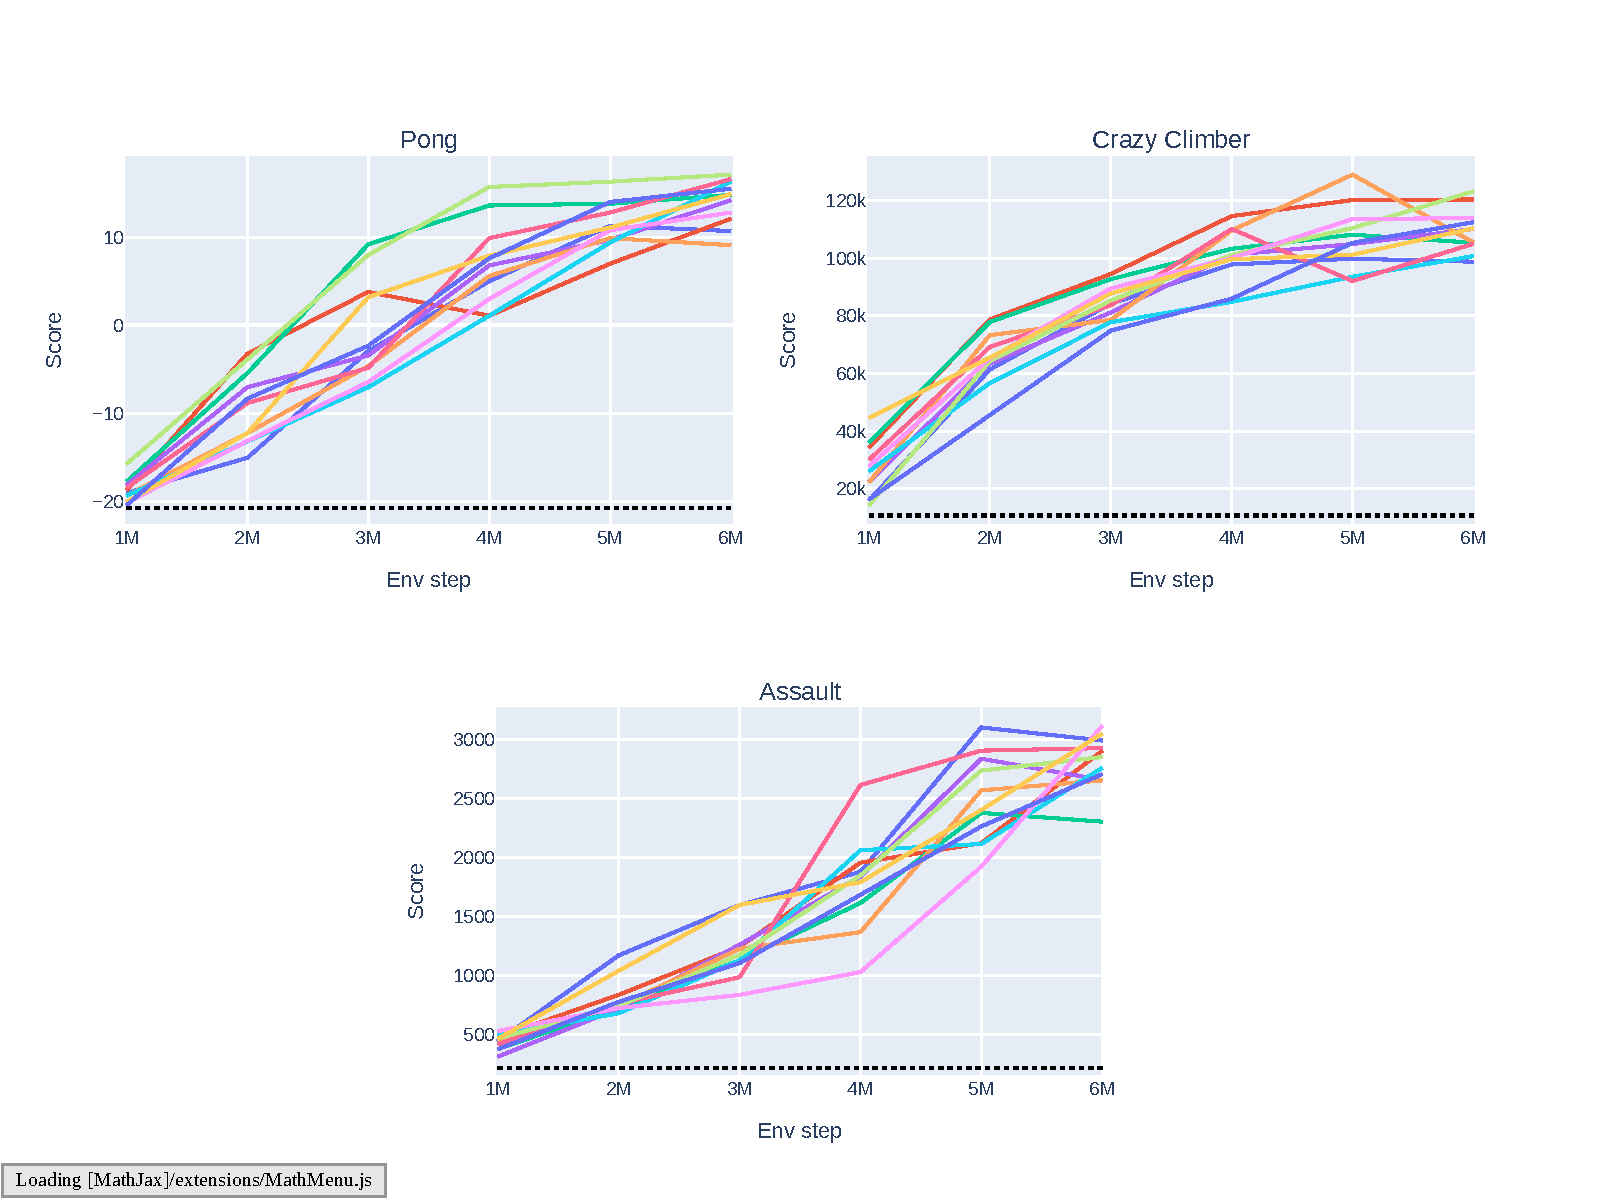
\includegraphics[width=\linewidth]{assets/perf_curves.pdf}
  \caption{Performance curves for a three-game subset of Atari-100k. The dashed line denotes mean score when choosing random actions. The colored lines represent different RNG seeds chosen. We use the scores provided by the authors of DreamerV2.}
  \label{fig:a100k_mono_perf}
\end{figure}

\subsection{Na\"ive speedup test}

Let us begin with the simplest way to speed up the learning process - increasing the frequency of optimization steps without any other changes.

\paragraph{Setup} Base DreamerV2 training recipe begins with a prefill of $P = 200 \times 10^3$ and continues until the total step count is $T = 200 \times 10^6$. The latter loop consists of $E = 64$ env steps (at the frame skip value of $4$, this corresponds to $16$ agent steps) and a single optimization step. As discussed previously, we replace $T$ by $6.4 \times 10^6$. With that, we can parametrize the recipe as follows: begin with a prefill of $P = \max((3 \times 10^3)E, 20 \times 10^3)$ env steps, and continue until $\max(10^5 E, 400 \times 10^3)$ env steps, making an optimization step every $E$ env steps. Then, setting $E$ to $64$ roughly corresponds to the original training setting, and until $E \geq 4$ the number of total optimization steps is constant while the total number of env steps decreases. For $E < 4$, the number of optimization steps increases, since we keep the total number of env steps at $400 \times 10^3$.



\vskip 0.2in
\bibliography{thesis}

\end{document}